\clearpage
\section{Lancer les expériences depuis un Terminal}
\label{sec:experiences}
Les fichiers sous \sel{exemples/} donnent des configurations relisibles. Les modes \sel{run}, \sel{compare}, \sel{video} et \sel{terrain} utilisent la même classe de paramètres depuis une image Pharo sans interface. Exécutez les commandes depuis le dossier de l'atelier. Adaptez le chemin de la VM et celui de l'image en fonction de l'installation.

\begin{lstlisting}
bash lancer-lot.sh "$VM_PHARO" "$IMAGE_PHARO" \
  exemples/legacy-sose.json ./resultats/legacy run

bash lancer-lot.sh "$VM_PHARO" "$IMAGE_PHARO" \
  exemples/comparaison-synthetique.json ./resultats/comparaison compare
\end{lstlisting}

Avec le lanceur de l'image installée, vous pouvez aussi utiliser ce raccourci.

\begin{lstlisting}
atelier="$HOME/sose-propre"
"$atelier/lancer.sh" lot \
  "$atelier/exemples/comparaison-synthetique.json" \
  "$atelier/resultats/comparaison" compare
\end{lstlisting}

Le fichier \sel{legacy-sose.json} rejoue le modèle SoSe historique. Conservez le mode de perception du scénario, les événements et la graine pour comparer une version de l'image à une autre. Testez les lois et hypothèses alternatives avec \sel{comparaison-synthetique.json}, où le parcours est défini en géométrie plane. La boucle fournit les intersections nécessaires à la reconstruction angulaire, y compris en l'absence de polygone WGS84.

\begin{lstlisting}
| options sortie |
options := SoSeAtelierParameters exampleComparison.
options
    at: #distanceWeight put: 2.0;
    at: #bearingHalfAngle put: 180.0.
options writeTo: FileLocator workingDirectory / 'comparaison.json'.
options := SoSeAtelierParameters readFrom:
    FileLocator workingDirectory / 'comparaison.json'.
sortie := FileLocator workingDirectory / 'comparaison'.
options runComparisonInto: sortie.
\end{lstlisting}

Pour utiliser la même configuration sur un terrain, sélectionnez un exemple avec \sel{terrainExample:} ou associez un MNT avec \sel{terrainDirectory:} et un parcours via \sel{path:}. Les \sel{Point} d'un parcours WGS84 utilisent `longitude@latitude'. Le mode \sel{video} requiert un terrain avec une grille préparée. Le JSON de paramètres utilise le format \sel{sose-atelier-parameters}, version 1. Un chemin de terrain relatif est résolu depuis le dossier du fichier JSON. L'exemple synthétique sert à comparer les lois avec un protocole stable. Simulez une fois par variante et comparez le maximum et l'écart-type des espacements, la vitesse et les parts d'observations refusées. Gardez constantes la graine, la portée, la cadence d'intégration et les vitesses bornes lorsque vous isolez l'effet d'un paramètre.

\subsection{Préparer une grille et lancer une vidéo}
Le fichier \sel{exemples/crozon-video.json} rejoue la grille côtière embarquée, avec un intervalle ralenti entre les tiks 10 et 15. Il sert à vérifier FFmpeg et le rendu avant de générer un nouveau terrain.

\begin{lstlisting}
bash lancer-lot.sh "$VM_PHARO" "$IMAGE_PHARO" \
  exemples/crozon-video.json ./resultats/crozon video
\end{lstlisting}

Depuis un Playground, fournissez la boîte géographique sous la forme ouest, sud, est, nord. Dans cet exemple, les quatre points du parcours sont conservés avec la grille. Retirez l'appel \sel{path:} pour calculer la grille avant de tracer le parcours.

\Needspace{14\baselineskip}
\begin{lstlisting}
| p destination |
p := SoSeAtelierParameters new
    terrainBounds: #(-4.56 48.22 -4.44 48.32);
    path: { -4.54 @ 48.25. -4.47 @ 48.25.
            -4.46 @ 48.28. -4.50 @ 48.30 };
    gridStep: 50;
    terrainMargin: 300;
    terrainSource: #copernicus;
    heightAboveGround: 150;
    fieldOfView: 55;
    yourself.
destination := FileLocator home / 'crozon-mission'.
p prepareTerrainInto: destination.
p writeTo: FileLocator home / 'crozon-mission.json'.
\end{lstlisting}

\begin{lstlisting}
bash lancer-lot.sh "$VM_PHARO" "$IMAGE_PHARO" \
  "$HOME/crozon-mission.json" ./resultats/crozon video
\end{lstlisting}

Pour préparer la grille directement depuis un JSON, utilisez le mode \sel{terrain}. Le dossier de destination devient le dossier de MNT, avec un fichier \sel{parametres.json} prêt à relire. Pour un rendu du jeu livré en un raccourci, \sel{terrainExample: 'crozon'} charge la grille et le tracé fournis, et \sel{displayAt: \#background put: \#planIgn} sélectionne le fond. \sel{playbackAt:put:} ajoute les options de lecture \sel{normalRate}, \sel{slowRate}, \sel{stride}, \sel{interval} ou \sel{hotspot}. \sel{metricZone:} définit le rectangle de mesure optique indépendamment du ralenti.

\clearpage
\subsection{Lire les résultats d'une comparaison}
Les paramètres de voisinage et le poids des écarts répondent à deux questions distinctes. Le poids règle l'intensité de la correction quand les écarts observés sont déséquilibrés. Le demi-angle de gisement règle où les observations angulaires peuvent être produites. Les métriques de perception montrent combien de fois la loi a effectivement reçu les entrées nécessaires. Une comparaison des trajectoires seule laisse cette information implicite.

\begin{figure}[ht]
\centering
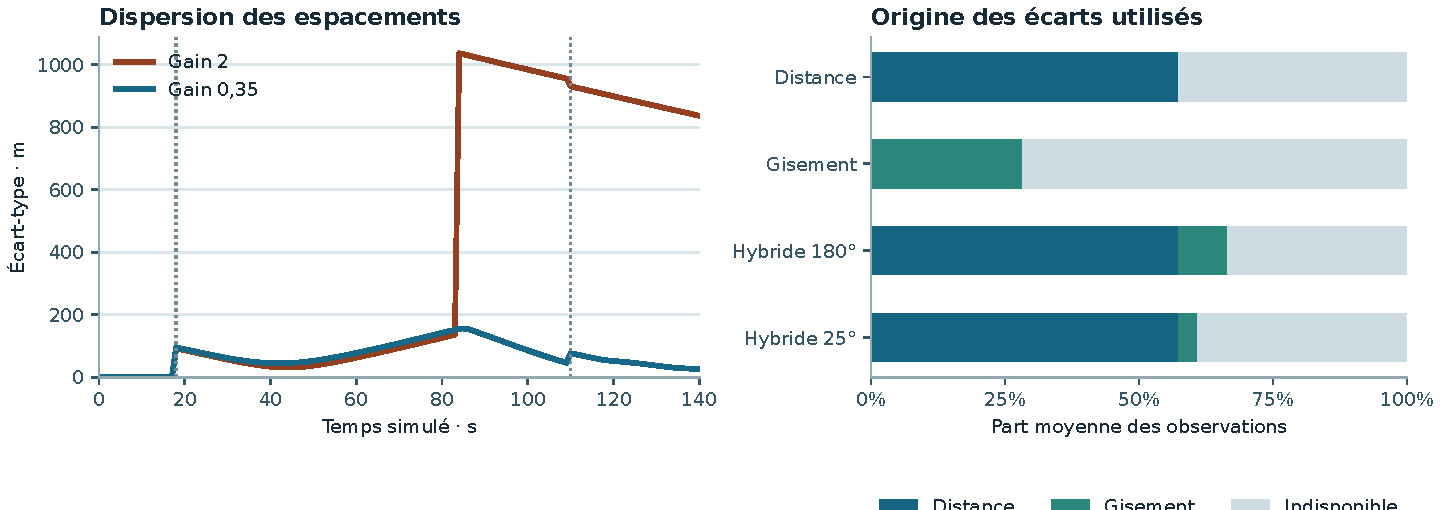
\includegraphics[width=\linewidth]{comparaison.pdf}
\caption{Résultats de Pharo 14 sur la boucle synthétique de 4 km avec 12 drones au départ et un tik de 1 s. Pointillés aux tiks 18 et 110 pour le retrait et l'entrée. Le retrait des mesures de distance aux tiks 25–84 et du gisement aux tiks 45–69 est commun à tout le lot.}
\end{figure}

Le lot écrit un dossier par variante avec son JSON et sa série \sel{simulation-timeseries.csv}, et un tableau \sel{comparaison.csv}. Les résultats livrés sous \path{exemples/resultats-reference/} servent à vérifier le rejeu. Dans le jeu perturbé, le gain 0,35 réduit l'écart-type final de 837 m à 27 m sur l'hybride. Le délai de revisite estimé au dernier état passe de 229,1 s à 65,5 s. Le demi-angle de 25° fait baisser la part des observations angulaires de 9,0\,\% à 3,4\,\% dans l'hybride. Cette ouverture n'a pas changé la part des observations directes. Les valeurs décrivent cette trajectoire, cette graine et ces indisponibilités.

Avec le même retrait et la même entrée, la variante \ui{Capping avec revisite} dépasse encore l'objectif de 32 s au dernier état. La boucle géométrique contient des mesures d'espacement et une estimation de revisite sur l'anneau.

\textbf{Lois à l'équilibre.} Pour isoler l'effet du délai embarqué, exécutez le mode \sel{compare} avec \sel{exemples/revisite-equilibre.json}. Ce jeu garde les 12 drones initialement espacés de 333 m et les observations directes disponibles pendant 140 tiks. Le tableau reprend les résultats finaux pour les trois lois en mode hybride.

\begin{tabularx}{\linewidth}{@{}Yrrr@{}}
\toprule
Variante & Vitesse moyenne & Délai estimé & États au-delà de 32 s \\
\midrule
Capping & 5,00 m/s & 66,67 s & 141 \\
Capping révisé & 10,00 m/s & 33,33 s & 141 \\
Capping avec revisite & 10,42 m/s & 32,00 s & 8 \\
\bottomrule
\end{tabularx}

Pour une comparaison optique, fixez la loi et le scénario, rejouez l'historique à deux hauteurs et exportez \sel{opticalCoverageRatio} et \sel{freshCoverageRatio} sur la même grille. Pour comparer le retour de service après un retrait et un renfort, figez les réglages d'affichage, activez les retraits et ralentissez une fenêtre centrée sur chaque événement. Comparez aussi dans le CSV le délai entre l'événement et le retour au-dessus de la cible sur la même zone.
